


\section{Prepacking}
\label{sec:prepacking}


The first step in our placement flow is \textbf{prepacking}. 
Recall from the 7-Series architecture that there are certain multi-cell structures that must adhere to certain placements constraints to ensure legality, and by design, to minimize wirelength. 
The job of the prepacker is to traverse the raw EDIF netlist, detect these multi-cell structures, and consolidate these cells into clusters or groups of clusters that naturally reflect these placement constraints. 

Recall that \texttt{CARRY4} chains must necessarily be placed vertically and consecutively across a column of SLICEs in ascending order. 
Likewise, \texttt{DSP48E1} cascades must necessarily be placed vertically and consecutively across a column of \texttt{DSP48E1} Sites in ascending order. 
A LUT-FF pair may be placed freely, but should be placed in the same lane within the same SLICE to minimize wirelength.

The raw EDIF netlist only tells us the list of nets and the cell ports that they connect to. 
It does not report the presence of any multi-cell structures (\texttt{CARRY4} chains, etc.). 
Thus, we must traverse the netlist to detect these multi-cell structures and store that structure information in a class we will call \texttt{PrepackedDesign}.

The code snippet in \ref{lst:carry_chains} shows how one can detect and collect these \texttt{CARRY4} chains in Figure \ref{fig:carry_chain_traversal} using RapidWright. 
We first collect the cells in the design that are of type \texttt{CARRY4}, then iteratively traverse their Carry-Out (\texttt{CO}) to Carry-In (\texttt{CI}) nets to find incident \texttt{CARRY4} cells.
Each \texttt{CARRY4} chain has an anchor cell and a tail cell where the chain terminates.
The anchor is found when the \texttt{CI} net connects to Ground (\texttt{GND}), while the tail is found when the \texttt{CO} port is null. 
We can further detect if there are \texttt{LUT}s or \texttt{FF}s connected to the \texttt{CARRY4} cell and store that information in a data structure we will call \texttt{CarryCellGroup} as defined in figure \ref{fig:substages}.
This will help us in knowing which cells can be packed together into the same \texttt{Site} in the subsequent stages. 

Similarly, \texttt{DSP48E1} cascades can be found and collected by traversing the \texttt{PCOUT} \texttt{ACOUT} and \texttt{BCOUT} nets.
\texttt{LUT-FF} pairs can be found by inspecting the LUT output (O) net and checking for FF input (DI) ports. 
We can bucket these LUT-FF pairs by finding the set of unique \texttt{CE} \texttt{SR} net pairs to know which group of LUT-FF pairs can be placed within the same \texttt{Site}. 

The overall goal of prepacking is to detect the presence of these multi-cellular structures and consolidate that information into our \texttt{PrepackedDesign} object in preparation for the following Packing stage. 


\end{multicols}
{
    \centering
    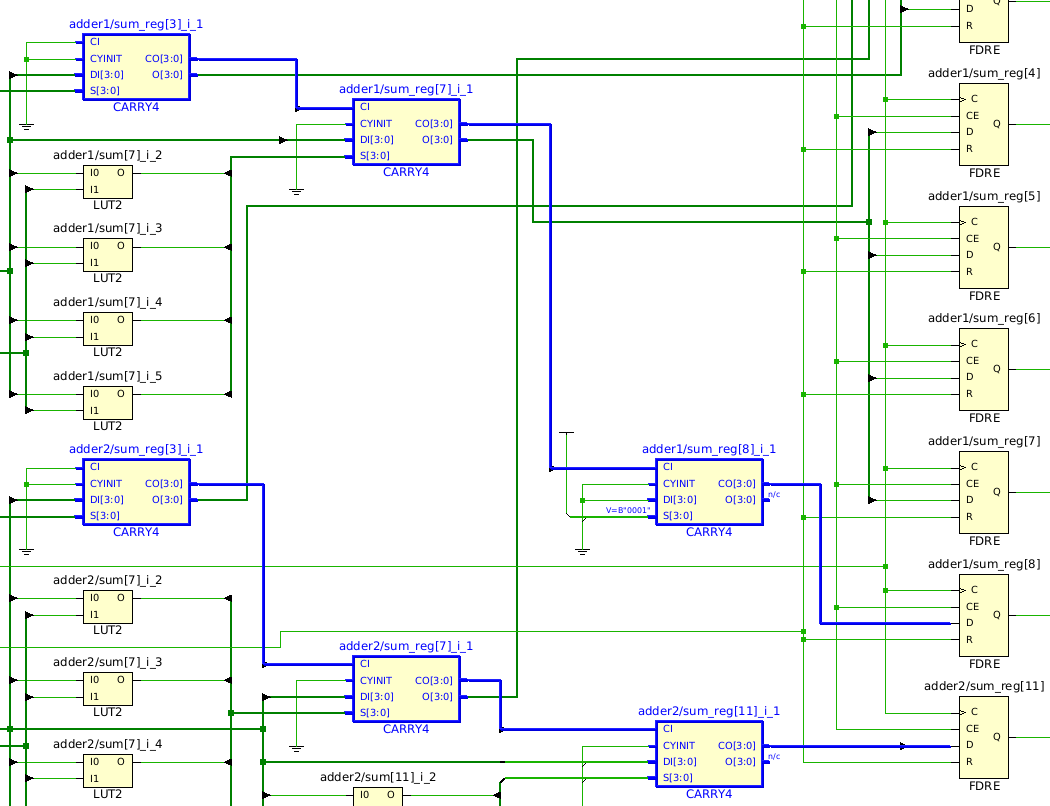
\includegraphics[width=0.8\columnwidth]{figures/carry_chain_traversal.png}
    \captionof{figure}{A netlist with two \texttt{CARRY4} chains, each of size 3}
    \label{fig:carry_chain_traversal}
}
\begin{multicols}{2}

\begin{lstlisting}[language=java, caption={Finding and storing carry chains.}, label={lst:carry_chains}]
Design design = Design.readCheckpoint("synth.dcp")
EDIFNetlist netlist = design.getNetlist();
List<EDIFCellInst> ecis = netlist.getAllLeafCellInstances();

// Select only the carry cells.
List<EDIFCellInst> carryCells = new ArrayList<>();
for (EDIFCellInst eci : ecis) {
    if (eci.getCellName().equals("CARRY4"))
        carryCells.add(eci);
}

// Find and remove carry chains until the list is empty
List<List<EDIFCellInst>> carryChains = new ArrayList<>();
while (!carryCells.isEmpty()) {
    // Set "currentCell" pointer to an arbitrary cell in list
    EDIFCellInst currentCell = carryCells.get(0);

    // Find this carry chain anchor.
    // Traverse the Carry-In (CI) to Carry-Out (CO) nets.
    // Anchor is found when net on the CI Port is Ground.
    while (true) {
        System.out.println(currentCell);
        // Access the CI port on this cell.
        EDIFPortInst sinkPort = currentCell.getPortInst("CI");
        // Access the net on this CI port.
        EDIFNet net = sinkPort.getNet();
        if (net.isGND()) {
            break; // Found this chain anchor!
        }
        // Get all ports on this net.
        List<EDIFPortInst> netPorts = net.getPortInsts();
        for (EDIFPortInst netPort : netPorts) {
            // Access the port belonging to another carry cell.
            EDIFCellInst sourceCell = netPort.getCellInst();
            if (sourceCell.getCellName().equals("CARRY4")) {
                // Move the "currentCell" pointer
                currentCell = sourceCell;
                break;
            }
        }
    }

    // Now currentCell points at this chain's anchor.

    // Now traverse in the opposite direction to find the chain tail.
    // Tail is found when the CO Port is null.
    // Collect the chain cells into an ordred list.
    List<EDIFCellInst> currentChain = new ArrayList<>();
    currentChain.add(currentCell);
    while (true) {
        EDIFPortInst sourcePort = currentCell.getPortInst("CO[3]");
        if (sourcePort == null) {
            break; // Found this chain's tail!
        }
        EDIFNet net = sourcePort.getNet();
        List<EDIFPortInst> netPorts = net.getPortInsts();
        for (EDIFPortInst netPort : netPorts) {
            EDIFCellInst sinkCell = netPort.getCellInst();
            if (netPort.getName().equals("CI") &&
                    sinkCell.getCellName().equals("CARRY4")) {
                currentCell = sinkCell;
                // Add the cell to the chain list.
                currentChain.add(currentCell);
                break;
            }
        }
    }
    // Add currentChain to the list of chains
    carryChains.add(currentChain);
    // Remove currentChain from the list of cells
    carryCells.removeAll(currentChain);
} // end while()

// Print out the carry chains. 
for (List<EDIFCellInst> chain : chains) {
    for (int i = 0; i < chain.size(); i++) {
        EDIFCellInst carry = chain.get(i);
        if (i == 0) {
            writer.write("\nAnchor Cell: " + carry.getName() + 
                ", CellType: " + carry.getCellName());
        } else {
            writer.write("\n\tCell: " + carry.getName() + 
                ", CellType: " + carry.getCellName());
        }
    }
}
\end{lstlisting}

\end{multicols}
\begin{lstlisting}[caption={Code Printout}]
Anchor Cell: adder2/sum_reg[3]_i_1, CellType: CARRY4
	Cell: adder2/sum_reg[7]_i_1, CellType: CARRY4
	Cell: adder2/sum_reg[11]_i_1, CellType: CARRY4
Anchor Cell: adder1/sum_reg[3]_i_1, CellType: CARRY4
	Cell: adder1/sum_reg[7]_i_1, CellType: CARRY4
	Cell: adder1/sum_reg[8]_i_1, CellType: CARRY4
\end{lstlisting}
\begin{multicols}{2}
